\RequirePackage{fix-cm}
\documentclass[twocolumn]{svjour3}          % twocolumn
\journalname{Behavior Research Methods}


%\documentclass[jou,apacite]{apa6}
%\shorttitle{Online behavioral research with psiTurk}
%
%\twoauthors{Author One}{Author Two}
%\twoaffiliations{Institute of Psychology}{Freud's Institute}
%
%\abstract{psiTurk is really great and you should use it.}
%
%\rightheader{Online behavioral research with psiTurk}
%\leftheader{Online behavioral research with psiTurk}

\usepackage{listings}
\usepackage{color}
\usepackage{graphicx}
\usepackage{soul}
\usepackage{natbib}


\definecolor{dkgreen}{rgb}{0,0.6,0}
\definecolor{gray}{rgb}{0.5,0.5,0.5}
\definecolor{mauve}{rgb}{0.58,0,0.82}

\lstset{frame=tb,
  %language=Java,
  aboveskip=5mm,
  belowskip=5mm,
  showstringspaces=false,
  columns=flexible,
  basicstyle={\ttfamily},
  numbers=none,
  numberstyle=\tiny\color{gray},
  keywordstyle=\color{blue},
  commentstyle=\color{dkgreen},
  stringstyle=\color{mauve},
  frame=none,
  breaklines=true,
  breakatwhitespace=true
  tabsize=3
}

\begin{document}

\title{psiTurk: A framework for running behavioral experiments online}

\author{First Author         \and
        Second Author %etc.
}


%\authorrunning{Short form of author list} % if too long for running head

\institute{F. Author \at
              first address \\
              Tel.: +123-45-678910\\
              Fax: +123-45-678910\\
              \email{fauthor@example.com}           %  \\
%             \emph{Present address:} of F. Author  %  if needed
           \and
           S. Author \at
              second address
}

\date{Received: date / Accepted: date}

\maketitle

\begin{abstract}
Insert your abstract here.
\keywords{Online experiments \and open science}
\end{abstract}

\tolerance=5000

\section{Introduction}

Online experiments are growing in popularity in the behavioral sciences.
While they offer some exciting opportunities to researchers, they also pose 
a new set of challenges, both technical and experimental.

psiTurk is a framework of software and web services that addresses these challenges. 
It facilitates the creation, deployment, and sharing of web-based experiments on Amazon Mechanical Turk (AMT),
 which is currently the most common platform to run human experiments online.
It solves a number of technical requirements including serving an experiment on the web, saving experimental data, and restricting the participant pool according to the experimenter's needs. It also provides an interface with AMT to create and test new projects as well as to manage and
 pay participants.

The principal goal of this framework is thus to handle common technical challenges so that researchers can focus on the development and dissemination of online experiments.
In this paper we present a high-level overview of the psiTurk framework and its advantages for running web-based experiments.
We begin with an overview of web-based experiments, the AMT platform, and the specific challenges that psiTurk is designed to address.
We then step through the core functionality of psiTurk and describe its role in an experimenter's workflow.
Finally, we consider some future directions for psiTurk and online experimentation in general.


\section{Web-based behavioral research}
It is easy to see why online experiments are an attractive option for behavioral scientists.
Compared to traditional methods of experimentation in the laboratory
they allow researchers to collect large data sets in a fraction of the time and at much lower cost.
At the same time, they also open up a completely new set of web-based tools that  can be used to
design the look and flow of an experiment and that far exceed the capabilities
of traditional experiment software.
They also cater to a wide range of needs from simple surveys to more complicated interactive interfaces,
 or even multi-player games.

Still, there exists a range of hurdles that researchers need to tackle when running experiments
online, some of which might altogether bar some scientists from adopting online experimentation.
 To find out more the specific needs and challenges we conducted a survey in early 2014 of behavioral 
 researchers regarding online experimentation. 

\subsection{Survey of researchers' needs}
 We collected responses from 201 researchers in psychology (58\%),
linguistics (16\%), marketing (7\%), neuroscience (6\%), and economics (4\%), most of whom had some
experience collecting behavioral data online in their labs (85\%).

These researchers showed a clear interest in online data collection. Nearly all listed fast data
collection (98\%) and large sample sizes (93\%) as benefits of online data collection, with most
interested in the potential for lower costs (75\%) and a more diverse population (60\%) as well. Nearly
40\% stated that they treat papers reporting data collected online identically to that collected in
a lab.

\begin{figure*}[tp]
\centering
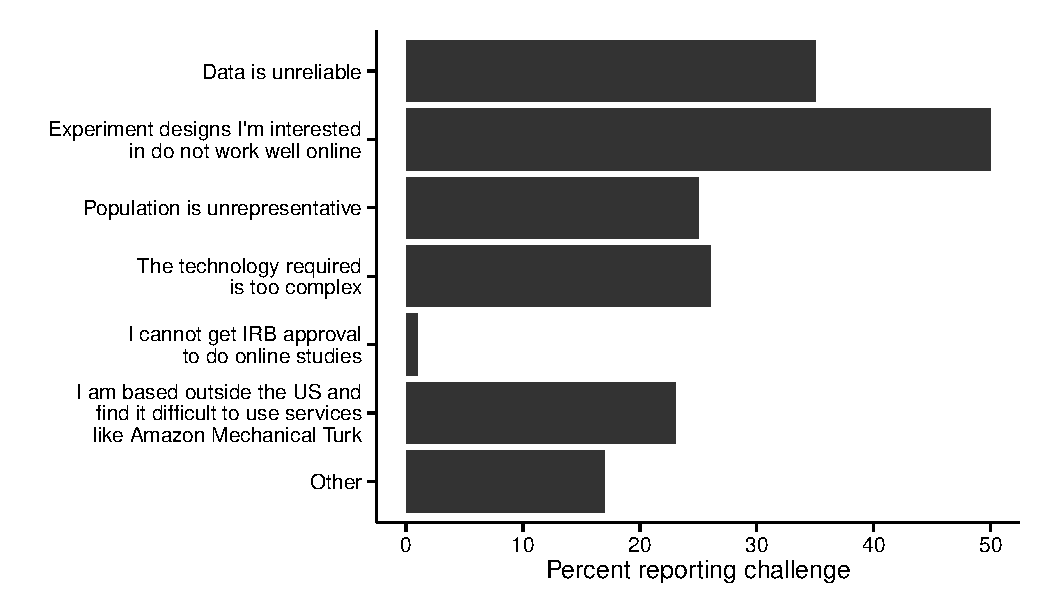
\includegraphics[scale=.75]{figures/challenges.pdf}
\caption{Challenges faced by 201 researchers who completed our survey on collecting behavioral data online.}
\label{fig:challenges}
\end{figure*}

Respondents also felt that online data collected presented a set of unique challenges, as shown in
Figure~\ref{fig:challenges}. Some felt that data collected online was unreliable (35\%) or the
population unrepresentative (25\%). Many felt that experiment designs they were interested in did
not work well online (50\%), or that web technology is too complex (25\%), and researchers based
outside the US reported difficulty using services like Amazon Mechanical Turk (23\%).


The majority of respondents (56\%) listed Qualtrics, a service for conducting online surveys, as the tool they
were currently most likely to use, but most (79\%) expressed interest in being able to run full
experiments including multiple, trials, fixation crosses, etc. The vast majority (94\%) reported
interest in new tools that simplified online data collection.


\subsection{Amazon Mechanical Turk} 

Amazon Mechanical Turk (AMT) is an online platform that lets you post a wide variety of tasks to a large pool of participants. People
who complete tasks, so called \emph{HITs} (Human Intelligence Tasks), are called \emph{workers}, people who post tasks are called
\emph{requesters}.
Instead of spending weeks to run experiments in the lab, AMT lets you collect data from a large number of workers within a couple of hours.
Beyond providing a platform to connect requesters and workers, AMT places few restrictions on the type of work that can be requested and the amount paid per HIT.
Workers are paid a fixed amount for each HIT they complete which is determined by the requester.

From a worker's perspective, the AMT website provides an up-to-date listing of HITs that are available, with a title, brief description, and payment amount.
A worker can click on a HIT to see its full \emph{advertisement} (an embedded webpage that is either hosted by
Amazon or the requester) and decide to accept the HIT. 
Accepting a HIT implies that they are reserving the ability to complete it within a timeframe specified by the requester.
The HIT itself can then be completed either on a requester's own hosted service, or on the AMT website itself through the use of customized templates.
Upon completion, the worker ``submits" the HIT, after which point the completed work must be approved by the requester before they are compensated.
In addition, some HITs offer bonus payments that are determined by the requester based on a worker's performance.

From a requester's perspective, AMT provides a web-based interface for creating/managing HITs and approving work that has been submitted.
In addition, they offer a ``sandbox" version of the platform in which HITs can be tested without paying live participants.

For basic tasks like surveys and open text fields, AMT offers a range of built-in templates that can be customized using the AMT website.
However, the degree of customization is limited for these templates. 
In particular, they do not support advanced experimental logic that is common to many psychology experiments (e.g., adapting the presentation of stimuli based on performance, or counterbalancing across a number of experimental variables).
For these kinds of tasks, a requester can provide a link to their own hosted service which runs the experiment, saves the data, and only interfaces with AMT at the beginning of the task (receiving basic information about the worker) and at the end of the task (sending confirmation that the task has been completed).

Thus, these ``external HITs" enable a much wider range of experiments at the cost of additional technical requirements.
psiTurk is designed to handle many of these requirements so that researchers can efficiently run experiments that are hosted externally.
% Specifically, it allows you to:
% 1. Run a web server for your experiment
% 2. Test your experiment
% 3. Interact with AMT to recruit, post HITs, filter, and pay participants (AMT workers)
% 4. Manage databases and export data


\subsection{What problems does psiTurk solve?}
To address the needs and concerned that survey participants mentioned, the psiTurk platform
 offers four key services.


\subsubsection{Interface to AMT}
psiTurk provides an easy to use interactive command line tool that can be used to 
interact with AMT without ever having to use the AMT website.  
The command line tool can be used to create and manage HITs, both live and in the AMT sandbox 
(AMT's testing environments for HITs before they go live), and to pay workers for
participating. Besides the basic payment that every worker receives for completing a HIT
it also has the capability to give automated bonus payments to participants based on a function
designed by the experimenter. This feature is particularly helpful since the AMT website
requires bonuses to be entered by hand for each participant individually.


\subsubsection{Technical complexity and security}
psiTurk reduces some of the main technical challenges that researchers face by providing a 
web server and basic data base to host an experiment and store participants' data. 
It also solves one very specific problem by providing a secure ad server that can
be used to serve the advertisements that workers see on the AMT website. Without  a secure server
 ads would not display on AMT and thus the ad server servers as a bridge between AMT and 
 a researcher's local computer. \hl{Someone may have to check if this is true :)} 
While providing a basic server and database, psiTurk also allows researchers to add custom
server routes or alternative databases that can be tailored to their specific needs. 

% Includes industry standards (Bootstrap, jQuery, d3, etc)

\subsubsection{Recruiting, filtering, and instructing participants}
Finally, psiTurk also has a range of features of particular interest to behavioral researchers
running controlled experiments. 
For example, it offers basic capabilities for assigning workers to different experimental conditions 
and counterbalancing features of the experiment. It also provides  a rage of templates
for common experiment building blocks (e.g., consent form, debriefing, instructions).
In addition, it allows experimenters to filter workers for example to exclude certain devices, platforms, or browsers, 
or to prevent the same worker to take a current or previous HIT repeatedly.


\subsubsection{Coding the Experiment}
In general, the psiTurk framework is \emph{not} designed as a programming interface for building the actual experiment.
That is, it requires that the experimenter knows some basic JavasScipt, HTML, and CSS to code the logic and looks of a new study.
Having said that, psiTurk does include its own JavaScript library, which provides helpful functions for recording data and sending
it back to the server, preloading pages and images, as well as some basic functions for looping through instruction screens. These
features should alleviate some of the most painful aspects of coding your own experiment and allow the researcher to focus
on the task logic and design instead. psiTurk also ships with a complete working example task that can be used as a template for 
new projects.


\subsection{Remaining challenges}
Some of the concerns raised by survey respondents are inherent to online data collection and therefore psiTurk does
not address them.
It is worth pointing out however that there exists some work on data reliability - one of the greatest worries that was found
in the questionnaire - that successfully replicates a wide range of classic cognitive psychology findings using AMT data~\citep{crump2013evaluating}. Interestingly, this study also found that increasing worker payment had no effect on reliability, suggesting that even 
at low payment levels data quality was high. 

On the other hand, there clearly exist experimental protocols that simply are not amenable to online
experimentation. Experiments that require very fine-grained temporal control over stimulus presentation, for example, 
may be unsuited because even modern browsers will not be able to reliably display content fast enough if the presentation time
becomes too short~\citep{crump2013evaluating}.
Similarly, any experiment that requires  control over a participant's screen size, resolution, or distance
from the screen will be problematic due to the uncontrolled nature of participants' environment. One advantage of psiTurk is that
it automatically collects data on worker's interaction with the experiment window, that is, if and when the window was resized and
if and when the user switched tabs or windows. This might help to at least get some grasp on a worker's level of distraction while completing
the task. 


% Requires careful consideration depending on the specific experimental design.
We will continue to discuss these challenges at the end of the paper.





\section{Overview of the psiTurk system}

The structure of the psiTurk system is shown in Figure X.

In this section we highlight important functions of each component.
Complete documentation and tutorials are available at http://psiturk.org/docs, including instructions for installing the software.

\subsection{Configuration and project structure}

After creating an Amazon Web Services account, a researcher must obtain credentials (a \emph{key ID} and a \emph{secret key}) that are saved in a global configuration file \texttt{.psiturkconfig}.
When psiTurk runs for the first time this file is automatically created in the user's home directory, but the user's AWS credentials must be added in order for psiTurk to interact with AWS.
Additionally, an account (and associated pair of keys) on the psiTurk.org website is required to allow posting of ads on the Ad server.
These credentials (obtained from a user's psiTurk profile page) are also placed in \texttt{.psiturkconfig}.

This global configuration is used whenever psiTurk is run, allowing multiple experiments (each residing in its own directory somewhere on the user's system) to rely on the same AWS and psiTurk accounts, or to share other common configuration options as desired.

A new psiturk project can be initialized in the current directory using:

\begin{lstlisting}
$ psiturk-setup-example
\end{lstlisting}

\noindent which creates a new directory containing an example experiment.
The project directory contains the following: \\


\noindent \texttt{config.txt}: This file contains settings for the current experiment, including:

\begin{itemize}
\item Metadata about the experiment that is displayed to workers on the AMT website (title, description)
\item Restrictions on which workers can accept the HIT, including geographic location (e.g., limiting to US workers only), AMT-specific qualifications (e.g., a worker's proportion of past work that has been approved), and web browsers that are permitted.
\item Database setup (Sqlite by default)
\item Server parameters
\item Task parameters
\end{itemize}


\noindent \texttt{custom.py}: Within Flask web framework, possible to add custom routes so that server-side functionality can be added to the psiTurk web server.
Cite some examples. \\ 

\noindent \texttt{participants.db}: If Sqlite is used (on by default), this file will be the database. \\

\noindent \texttt{server.log}: A log file containing any messages from the experiment server (not from the actual experiment code!) \\ 

\noindent \texttt{static/} directory: Experiment files, including Javascript, CSS, and images \\

\noindent \texttt{templates/} directory: HTML files associated with experiment \\


Setting up a new experiment thus entails 1) editing the settings in \texttt{config.txt}, followed by 2) modifying the contents of the \texttt{static} and \texttt{templates} directories to program the experiment.
The remaining files are only necessary in order to debug server errors (\texttt{server.log}), add new server-side functionality (\texttt{custom.py}), or to access saved data (\texttt{participants.db}).

To run your experiment in a web browser you need to have at least some basic web programming skills (especially using HTML, CSS, and JavaScript).
Once you mastered the basics, you can take advantage of the vast number of libraries and tools that can help you to build sharp and sophisticated experiments with the support of a large community of users.


\subsection{Command line interface: Managing HITs and serving the experiment}

PsiTurk runs as a command line interface (CLI) within a standard terminal window.
There are several advantages to designing psiTurk as a simple CLI beyond its efficiency of use. This
design makes the user-interface code clear and easy to read and write, allowing newcomers to quickly
understand and contribute to the open-source project. Integrating a new feature into the interface
is as simple as describing the syntax and functioning of a new command. The CLI also ensures that
psiTurk is easy to interact with not just on a laptop or desktop but also on a remote server or in
the cloud, where users may have terminal-only access.
 
Tab completion makes it quick to type commands, and the \texttt{help} command can be used to show
details on the usage of any command. 
The straightforward and consistent syntax of the CLI allows
users to perform a wide variety of tasks--from creating HITs and paying workers, to launching Amazon
Web Services database instances, to opening an experiment in a browser for debugging--that
would otherwise be spread across a number of websites and programs. 

Entering
\texttt{psiturk} at the command line in any directory containing a psiTurk project launches the
psiTurk CLI.
The psiTurk CLI features a colorized prompt that provides important information at a glance, including
whether the server is running, the current mode (``live" or ``sandbox", and the number of HITs currently running on AMT:

\begin{lstlisting}
[psiTurk server:off mode:sdbx #HITs:0]$
\end{lstlisting}

\noindent In some examples below, this prompt is truncated as \texttt{[psiTurk]\$} to indicate commands that occur within the psiTurk CLI, while commands that are entered on the command line are preceded simply by \texttt{\$}.


\subsubsection{Managing HITs}
Commands are organized into groups based on their function, following a general ``\texttt{command subcommand
arguments}'' format. For example, one can create a HIT by typing 

\begin{lstlisting}
[psiTurk]$ hit create <# assignments> <$ amount> <duration>
\end{lstlisting}

What happens after you create a HIT?

List any existing HITs with:

\begin{lstlisting}
[psiTurk]$ hit list --active
\end{lstlisting}


\subsubsection{Serving an experiment}

The experiment server is started using

\begin{lstlisting}
[psiTurk]$ server on
\end{lstlisting}

\noindent This opens the port specified in the project configuration file.
The experiment server will then respond to incoming requests, assuming that the port is publicly accessible.
This requires a static IP to prevent the experiment's URL from changing.
Users without a static IP address can use a dynamic DNS service to forward requests to their dynamic IP.
If the system running psiTurk is behind a router, the router must be configured to forward requests on the same port.

During the development of an experiment, the current code can be tested using:

\begin{lstlisting}
[psiTurk]$ debug
\end{lstlisting}

\noindent which will open a new browser window in which the current experiment can be tested.

Can restart the server with \texttt{server restart} or open the server log with \texttt{server log}. 

Easily switch between AMT's sandbox and live site.

In most cases, a user of the
psiTurk CLI will never have to log into the MTurk website except to add money to their MTurk
requester account.


\subsection{The Ad server}

PsiTurk helps an experimenter in both hosting the ad and delivering the experiment.
First, PsiTurk provides a cloud service at \texttt{psiturk.org} for serving ads to workers.
This service serves the ads with appropriate SSL certificates, something which can be difficult on many server configurations.\footnote{SSL certification has recently become a requirement for hosting content within an \texttt{iframe} on \texttt{mturk.com}.}
Second, the PsiTurk web framework allows you to easily build and host your own experiment, running on your server or laptop and saving workers' data either to your own database  or to \texttt{psiturk.org}.
This gives experimenters complete flexbility in terms of content while also offering a suite of tools to make experiment development easy.

SSL hosted Ad Server removes need to deal with complex web security issues (https, data mining on workers) 
Participants recruited via Mechanical Turk first interact with your task via ads. Ads are simply the digital version of hanging a poster or flyer around your university building in order to recruit participants. Technically, ads are snippets of HTML code that describe what your task is about and what you're offering for compensation. As a result, they are the front line for any subject recruitment online. It's easy to overlook the importance of a good ad, and making that ad visible to as many participants as possible.




%Extendable Python based API: easily add new functionality
%
%Library of experiments you can adapt or replicate
%
%Fully open-source development helps catch bugs
%
%Since everything runs locally easy to debug/test (even w/o Internet!)
%
%Run experiments on local computer (via tunnel) (can run offline and online)
%
%Perfect for laboratory-based courses with undergrads (replicating studies)



\subsection{Javascript library \emph{psiTurk.js}}

The javascript library \emph{psiTurk.js} enables interaction with the server from the client-side (javascript) experiment code.
The goal of the library is to handle the most common functionality of psiTurk-based web experiments, without imposing any additional requirements on the structure or design of the experiments themselves.
Researchers can draw on a vast array of javascript libraries to design their experiment, while using psiTurk.js to save data and notify the server of changes in a participant's status.

Figure X shows javascript code from an experiment script (\emph{task.js}). 
\emph{psiTurk.js} currently performs the following functions:


\subsubsection{Tracking a participant's progress in an experiment} 

psiTurk records changes in a participant's status as they move through an experiment. 
Some of these status changes are automatic, e.g., when a participant is assigned to a condition or if they quit an experiment early. 
Two additional status changes are initiated by the client-side experiment code using psiTurk.js functions.
First, since experiments typically begin with an instructional phase, calling the function \texttt{psiturk.finishInstructions()} upon completion of this phase will save the participant's status as having begun the main experiment.
If the participant attempts to quit the experiment after that point, they will receive a warning that they will not be able to restart the experiment and may forgo payment.
Second, successful completion of the experiment is signaled by calling \texttt{psiturk.completeHIT()}, which closes the experiment and redirects the participant to the AMT page to submit their HIT.

\subsubsection{Saving experimental data} 

Experiment code can save data in two formats.
\texttt{psiturk.recordTrialData} takes any array of values as input and appends it to a list of ``trial" data.
This data structure is meant for sequential data that may be collected over the course of multiple trials or blocks, where each line corresponds to a new measurement.
However, the format of this data is defined by the experimenter and is saved in the database as a single JSON object.

In contrast, \texttt{psiturk.recordUnstructuredData} is used to record (key, value) pairs, where the key is uniquely defined within the experiment.
This format is useful for survey questions or other one-time measurements, e.g., (\emph{Age}: 24).

Importantly, both functions above simply record the data in the appropriate format on the client-side.
When the experimenter wishes to save the data to the server they call \texttt{psiturk.saveData}.

\subsubsection{Automatic recording of browser interaction}
 
One general shortcoming of web experiments is greater uncertainty about a participant's testing environment and engagement with the experiment.
Unlike lab computers where undesired behaviors can be prevented, a person is always able to close a web browser, switch to different applications, or change other aspects of their experience.
However, standard methods exist for recording many aspects of a user's interaction with a web browser, and this data can be useful for 1) tracking how an experiment was actually displayed, and 2) the level of a participant's engagement.

For example, although it is possible to set the initial size of a browser window, a web participant can change the dimensions of the window, potentially obscuring or altering how the experiment is displayed.
\emph{psiTurk.js} automatically records these changes in the size of the window.
Similarly, the experiment can choose to switch focus away from the experiment window (e.g., to another browser window or a different application).
\emph{psiTurk.js} automatically records every time that the experiment window loses and gains the participant's focus.
This ``event data" is automatically recorded and saved to the database whenever \texttt{psiturk.saveData} is invoked. \\


\emph{psiTurk.js} can also preload html pages and images.
Finally, it has a basic structure for presenting instructional pages.

\subsection{Experiment exchange}

A significant advantage of web-based experiments is the potential for low-friction replication and extension. 
The \emph{experiment exchange} (EE, found at http://psiturk.org/ee) facilitates the sharing of experiments that have been built to run using psiTurk, acting as an ``app store" for psiTurk-compatible designs.
Once an experiment has been completed, a researcher can submit the following information to register their experiment on the exchange:

\begin{enumerate}
\item A Github repository containing the experiment code
\item Metadata about the experiment, including a title, description, and keywords
\item The DOI for any paper describing the results of the experiment (if any)
\item The version of psiTurk that was used to run the experiment
\end{enumerate}


Metadata associated with an experiment allows other researchers to discover it through the psiTurk website.
A publicly available experiment can then be downloaded using the following command on the command line,

\begin{lstlisting}
$ psiturk-install <experiment-specific-id>
\end{lstlisting}

\noindent with the experiment-specific identifier found on the exchange page.
If psiTurk is already configured on the user's system, the downloaded experiment will run without further changes, and can then act as a starting point for direct replication or extensions.
Modified versions can then be re-run using the same population via AMT, thereby minimizing the potential for experimenter-specific biases.

Other initiatives (e.g., the Open Science Framework, https://osf.io) also aim to improve the transparency, reproducibility, and efficiency of research through centralized services, but are less focused on the specific technology involved in running online experiments.
In contrast, the psiTurk experiment exchange links together experiments that can be run within a common framework.
As a result, existing experiments can serve as examples to help new researchers learn to code for the web; they shorten the development time necessary (especially for popular experimental paradigms); and the exchange facilitates communication between researchers with similar interests.

\section{Limitations and future directions (TMG)}

As mentioned above, psiTurk faces some challenges inherent to all online data collection and may not be the right choice for
researchers that require a very controlled experimental setup. But what are the limitations of psiTurk specifically?

One restriction is that it's currently designed to only work with Amazon Mechanical Turk. A common worry with AMT is the unrepresentativeness of
its subject pool (in terms of demographics and geography), as well as the fact that certain experimental protocols are now too well-known 
to workers to guarantee naive
participants~\citep{chandler2014nonnaivete}. These concerns are often not relevant for basic psychology research, but some experimenters may nevertheless
look for alternatives to AMT. Many psiTurk features (i.e. the web server, data base, and psiturk.js) are general
enough to facilitate running experiments on other platforms, too, but it would require some customization of certain AMT-specific functionality. 
We hope that researchers who decide
to use psiTurk on another platform could contribute such changes to the github repository (https://github.com/NYUCCL/psiTurk) to make them
available to the community.


Another limitation is that psiTurk only runs on UNIX systems, like Linux and Mac OS, and can thus not be used on Windows computers. To meet this 
challenge, one option for Windows users is to use a cloud-based computing service to run psiTurk and host experiments. There exist
multiple free or low-cost options, such as Amazon Web Services (http://aws.amazon.com), or OpenShift (https://www.openshift.com). 
The installation steps and setup may diverge slightly from the standard procedure but 
 the psiTurk documentation already contains additional installation instructions for OpenShift. In the future, we hope to extend support  and 
documentation to a wider range of cloud computing options.

Another future direction is to extend the counterbalancing capabilities of psiTurk. Currently, the built-in counterbalancing algorithm
simply aims to assign participants equally to different cells.  However, this equal assignment method can be problematic if, for instance, 
one group has a higher drop-out rate than the others (a problem rarely encountered in the lab). 
In that case the high drop-out group will need to receive
more participants to equalize the difference and thus assignment probabilities will no longer be equal across groups. We are
currently working on alternative counterbalancing algorithms that keep assignment probabilities equal (which may then lead to unequal
number of participants) to avoid this problem. \hl{Not quite sure what the current status is here. May need updating and maybe mention PlanOut
if that's still relevant.}


One exciting prospect of running online experiments is to let multiple participants interact to study coordination
or group behavior. Currently psiTurk does not offer its own tool to facilitate such multi-person experiments, but we would like to
add support for it in the future, using web-sockets or other protocols that enable communication between users.

\hl{Some small features not mentioned yet:

Automate catch trials? How far did the worker get? Do we count them in the N? 

Limiting/throttling number of people doing the experiment at once

Video support}





% BibTeX users please use one of
\bibliographystyle{spbasic}      % basic style, author-year citations
%\bibliographystyle{spmpsci}      % mathematics and physical sciences
%\bibliographystyle{spphys}       % APS-like style for physics
\bibliography{psiturk}

\end{document}
